\documentclass[12pt,preprint]{aastex}

% has to be before amssymb it seems
%\usepackage{color,hyperref}
%\definecolor{linkcolor}{rgb}{0,0,0.5}
%\hypersetup{colorlinks=true,linkcolor=linkcolor,citecolor=linkcolor,
%            filecolor=linkcolor,urlcolor=linkcolor}

\usepackage{color}
\usepackage{url}
\usepackage{algorithmic,algorithm}
\usepackage{amssymb,amsmath}
\usepackage{graphicx}
\graphicspath{{figures/}}


%\usepackage{listings}
%\definecolor{lbcolor}{rgb}{0.9,0.9,0.9}
%\lstset{language=Python,
%        basicstyle=\footnotesize\ttfamily,
%        showspaces=false,
%        showstringspaces=false,
%        tabsize=2,
%        breaklines=false,
%        breakatwhitespace=true,
%        identifierstyle=\ttfamily,
%        keywordstyle=\bfseries\color[rgb]{0.133,0.545,0.133},
%        commentstyle=\color[rgb]{0.133,0.545,0.133},
%        stringstyle=\color[rgb]{0.627,0.126,0.941},
%    }

\newcommand{\foreign}[1]{{\it #1}}

\newcommand{\adhoc}{\foreign{ad hoc}}
\newcommand{\etal}{\foreign{et\,al.}}
\newcommand{\etc}{\foreign{etc.}}

\newcommand{\Fig}[1]{Figure~\ref{fig:#1}}
\newcommand{\fig}[1]{\Fig{#1}}
\newcommand{\figlabel}[1]{\label{fig:#1}}
\newcommand{\Eq}[1]{Equation~(\ref{eq:#1})}
\newcommand{\eq}[1]{\Eq{#1}}
\newcommand{\eqlabel}[1]{\label{eq:#1}}
\newcommand{\Sect}[1]{Section~\ref{sect:#1}}
\newcommand{\sect}[1]{\Sect{#1}}
\newcommand{\App}[1]{Appendix~\ref{sect:#1}}
\newcommand{\app}[1]{\App{#1}}
\newcommand{\sectlabel}[1]{\label{sect:#1}}


\begin{document}

\title{Multiband Periodograms of Astronomical Sources}

\newcommand{\escience}{1}
\newcommand{\uwastro}{2}
\author{Jacob T. VanderPlas\altaffilmark{\escience}}
\author{{\v Z}eljko Ivezi{\'c}\altaffilmark{\uwastro}}
\altaffiltext{\escience}{eScience Institute, University of Washington}
\altaffiltext{\uwastro}{Department of Astronomy, University of Washington}


\begin{abstract}
  This paper introduces a general method for least-squares spectral fitting of multi-band periodic data.
\end{abstract}

\keywords{
    methods: data analysis ---
    methods: numerical ---
    methods: statistical
}

\section{Introduction}

The detection and quantification of periodicity in time-varying signals is an important area of data analysis within modern astronomical surveys.
For evenly-spaced data, the {\it Schuster periodogram}, introduced in 1905, gives a quantitative measure of the periodicity of data as a function of the angular frequency $\omega$. For data $\{d_k\}_{k=1}^N$ measured at equal intervals $t_k = t_0 + k\Delta t$, the Schuster periodogram, which measures the spectral power as a function of the angular frequency, is given by
\begin{equation}
  \eqlabel{Schuster}
  C(\omega) = \frac{1}{N}\left| \sum_{k=1}^N d_k e^{i\omega t_k} \right|^2,
\end{equation}
and can be computed very efficiently using the Fast Fourier Transform.

Because astronomical observing cadences are rarely so uniform, many have looked at extending the concept of the periodogram. Most famously, \citep{Lomb76} and \citep{Scargle82} extended earlier work to define the {\it normalized periodogram}:
\begin{equation}
  \eqlabel{LombScargle}
  P_N(\omega) = \frac{1}{2\sigma^2}\left[
    \frac{\left[\sum_k(d_k - \bar{d})\cos\omega(t_k - \tau)\right]^2}
    {\sum_k \cos^2\omega(t_k - \tau)}
    +
    \frac{\left[\sum_k(d_k - \bar{d})\sin\omega(t_k - \tau)\right]^2}
    {\sum_k \sin^2\omega(t_k - \tau)}
\right],
\end{equation}
where $\bar{d}$ is the mean and $\sigma^2$ is the variance of the data $\{d_k\}$, and $\tau$ is the time-offset which makes $P_N(\omega)$ independent of a translation in $t$ \citep[See][for an in-depth discussion]{NumRec}. \citep{Lomb76} showed that this offset has a more important effect: namely, it makes $P_N$ identical to the estimate of harmonic content given a least-squares fit to a single-component sinusoidal model,

\begin{equation}
  \eqlabel{SingleModel}
  d(t) = A\sin(\omega t + \phi).
\end{equation}

This deep connection between spectral power and least squares fitting methods was solidified by \citep{Jaynes87}, who demonstrated that the normalized periodogram of Lomb and Scargle is a sufficient statistic for inferences about a stationary-frequency signal in the presence of Gaussian noise. Building on this result, \citep{Bretthorst88} explored the extension of these methods to more complicated models with multiple frequency terms, nonstationary frequencies, and other more sophisticated models within a Bayesian framework.

(Mention supersmoother and ARMA-based methods?)

A weakness with the above methods is that they require homogeneous measurements -- for astronomy data, this means that successive measurements must be taken through a single band. This has not been a problem for past surveys, as measurements are generally taken through a single photometric filter (e.g. LINEAR, ??), or in all bands at each observation (e.g. SDSS, ??). In such cases, past studies have generally relied on \adhoc{} methods such as a majority vote among multiple single-band estimates of the periodogram.

For future multicolor surveys such as LSST, this \adhoc{} approach will not be sufficient. In order to take advantage of the full available data, it would be desirable to have a single estimate of the periodogram which accounts for all observed data in a manner which is not dependent on the underlying spectrum of the object. We propose such a method below.


\section{Background: Matrix Formalism for Periodograms}

In this section we will give a quick quantitative introduction to the least squares fitting formulation of the normalized periodogram of \eq{LombScargle}. We'll denote our $N$ observed data points as
\begin{equation}
  D = \{t_k, y_k, \sigma_k\}_{k=1}^N
\end{equation}
where $t_k$ is the time of observation, $y_k$ is the observed value (typically a magnitude), and $\sigma_k$ describes the Gaussian errors on each value. Without loss of generality we will assume that the data $y_k$ are centered such that the measurements satisfy
\begin{equation}
  \eqlabel{ycentered}
  \frac{\sum_k w_ky_k}{\sum_k w_k} = 0
\end{equation}
where the weights are $w_k = \sigma_k^{-2}$.

\subsection{Stationary Sinusoid Model}
The Lomb-Scargle periodogram of \eq{LombScargle} can be derived from the normalized $\chi^2$ of the best-fit single-term stationary sinusoidal model given in \eq{SingleModel}. To make the problem linear, we can re-express the model in terms of the parameter vector $\theta = [A\cos\phi, A\sin\phi]$ so that our model is
\begin{equation}
  \eqlabel{simplemodel}
  M(t|\omega,\theta) = \theta_1\sin(\omega t) + \theta_2\cos(\omega t).
\end{equation}
We can find the maximum likelihood estimate of the parameters $\theta$ by minimizing the $\chi^2$ of the model, which is given by
\begin{equation}
  \chi^2(\omega) = \sum_k \frac{(y_k - M(t_k|\omega,\theta))^2}{2\sigma_k^2}.
\end{equation}
For the single-term Fourier model, it can be shown \citep[See, e.g.][]{ICVG2014} that
\begin{equation}
  \eqlabel{chi2_PN}
  \chi_{min}^2(\omega) = \chi^2_0[1 - P_N(\omega)]
\end{equation}
where $P_N(\omega)$ is the normalized periodogram given in \eq{LombScargle} and $\chi^2_0$ is the reference $\chi^2$ for a constant model, which due to the assumption in \eq{ycentered} is simply $\chi^2_0 = \sum_k (y_k/\sigma_k)^2$

These quantities can be expressed more compactly by defining the following matrices:

\begin{equation}
X_\omega = \left[
\begin{array}{cc}
\sin(\omega t_1) & \cos(\omega t_1)\\
\sin(\omega t_2) & \cos(\omega t_2)\\
\vdots & \vdots \\
\sin(\omega t_N) & \cos(\omega t_N)\\
\end{array}
\right];~~
y = \left[
\begin{array}{c}
y_1 \\
y_2\\
\vdots \\
y_N\\
\end{array}
\right];~~
\Sigma = \left[
\begin{array}{cccc}
\sigma_1^2 & 0 &  \cdots & 0\\
0 & \sigma_2^2 &  \cdots & 0\\
\vdots & \vdots &  \ddots & \vdots\\
0 & 0 &  \cdots & \sigma_N^2
\end{array}
\right]
\end{equation}

With these definitions, the model in \eq{simplemodel} is a simple linear product: $M(t|\omega,\theta) = X_\omega\theta$ and the model and reference $\chi^2$ can be written

\begin{eqnarray}
  \chi^2(\omega) &=& (y - X_\omega\theta)^T\Sigma^{-1}(y - X_\omega\theta)\\
  \chi^2_0 &=& y^T \Sigma^{-1} y
\end{eqnarray}

the normalized periodogram can be computed by finding the minimum of $\chi^2(\omega)$ via standard methods and plugging the result into \eq{chi2_PN} to find

\begin{equation}
  \eqlabel{LombScargle2}
  P_N(\omega) = \frac{y^T\Sigma^{-1}X_\omega(X_\omega^T\Sigma^{-1}X_\omega)^{-1}X_\omega^T\Sigma^{-1}y}{y^T\Sigma^{-1}y}
\end{equation}

For $\Sigma \propto I$, this expression is equivalent to \eq{LombScargle}.

While \eq{LombScargle} can be computed more efficiently than \eq{LombScargle2}, the matrix-based formulation has several advantages
\begin{enumerate}
  \item It is trivially extended for heteroscedastic and/or uncorrelated noise in the data $y_k$ by appropriately modifying the noise matrix $\Sigma$
  \item It is trivially extended to more sophisticated models by appropriately modifying the design matrix $X_\omega$.
  \item It is trivially extended to L2-regularized likelihoods by adding an appropriate diagonal term to $X_\omega^T\Sigma^{-1}X_\omega$ before inverting.
\end{enumerate}

\subsection{Lomb-Scargle with Floating Mean}

As an example of one of these generalizations, consider the {\it generalized Lomb-Scargle} method of \citep{Zechmeister09}. This adjusts the classic Lomb-Scargle algorithm by using a model with a floating mean, which can be more accurate for certain observing cadences:

\begin{equation}
  M(t~|~\omega, \theta) = \theta_0 + \theta_1\sin\omega t + \theta_2\cos\omega t
\end{equation}

While \citep{Zechmeister09} details a formalism to express this {\it generalized periodogram} model similarly to \eq{LombScargle}, in the matrix formalism all that is required is to add a column of ones to the $X_\omega$ matrix before computing the power via \eq{LombScargle2}.

\subsection{Truncated Fourier Models}
In a similar vein, the power for a truncated Fourier series model of any order can be constructed by extending the $X$ matrix with appropriate columns; for example, for a 2-term truncated Fourier fit with a floating mean we can write

\begin{equation}
X_\omega = \left[
\begin{array}{ccccc}
1 & \sin(\omega t_1) & \cos(\omega t_1) & \sin(2\omega t_1) & \cos(2\omega t_1)\\
1 & \sin(\omega t_2) & \cos(\omega t_2) & \sin(2\omega t_2) & \cos(2\omega t_2)\\
1 & \sin(\omega t_3) & \cos(\omega t_3) & \sin(2\omega t_3) & \cos(2\omega t_3)\\
\vdots & \vdots & \vdots & \vdots & \vdots \\
1 & \sin(\omega t_N) & \cos(\omega t_N) & \sin(2\omega t_N) & \cos(2\omega t_N)\\
\end{array}
\right]
\end{equation}

Plugging this $X$ matrix into Eqn.~\ref{eq:power} will give us the normalized periodogram associated with the two-term truncated Fourier model.

\subsection{Regularized Models}

Show how regularized models fit into this.


\section{Moving to Multiple Bands}

\begin{itemize}
  \item Write-out the linear model
  \item Demonstrate the matrix form of this
  \item Use light regularization
  \item Correspondance of the single-term multiband result to the weighted sum of single-band Lomb-Scargle results
\end{itemize}

\section{Examples}
\subsection{Simulated Example}

\begin{figure}
  \centering
  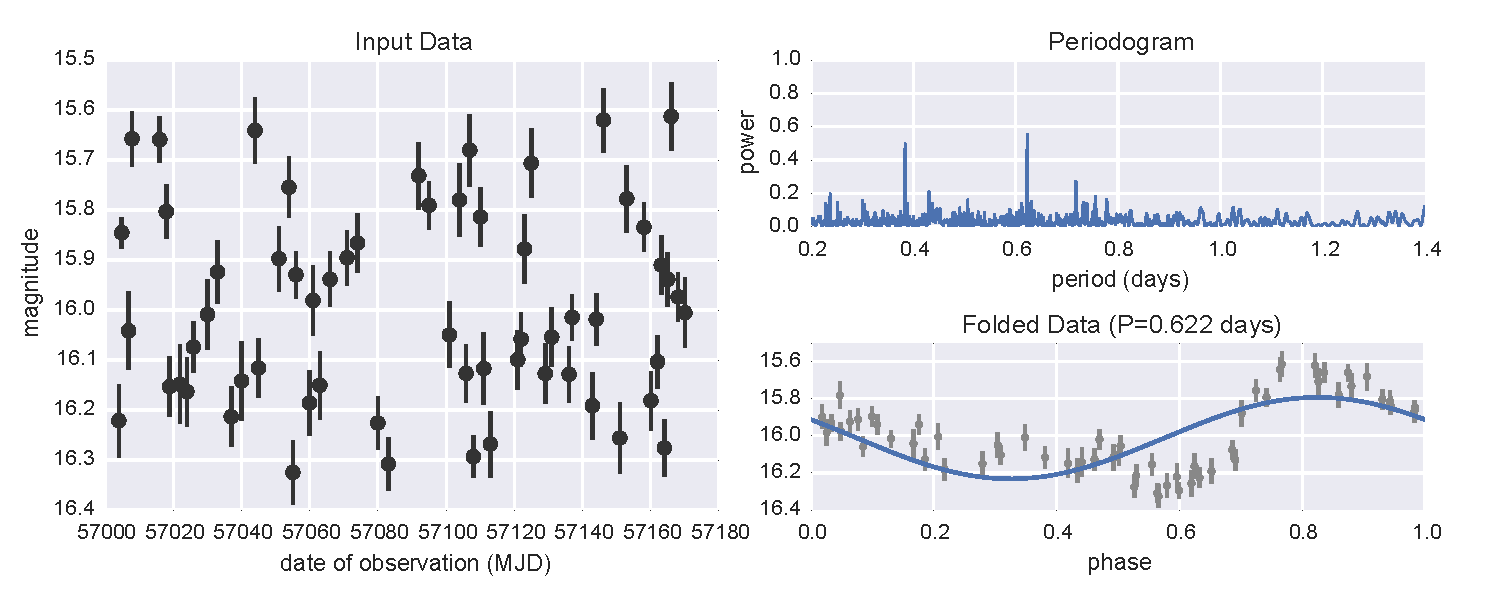
\includegraphics[width=\textwidth]{fig01.pdf}
  \caption{
    An illustration of the typical approach to multiband periodograms,
    in which each band is fit individually. The data consists of 60 coeval
    {\it ugriz} observations spread over 180 nights, and is based on an
    RR Lyrae template from \citet{Sesar2010}. With this much data in each
    band, individual periodograms can be constructed and compared to find the
    true period $P=0.622$ days. Note also the presence of aliasing typical
    in Lomb-Scargle periodograms, located at beat frequencies between the
    true Period and the 1-day observing cadence.
  }
  \figlabel{01}
\end{figure}

\begin{figure}
  \centering
  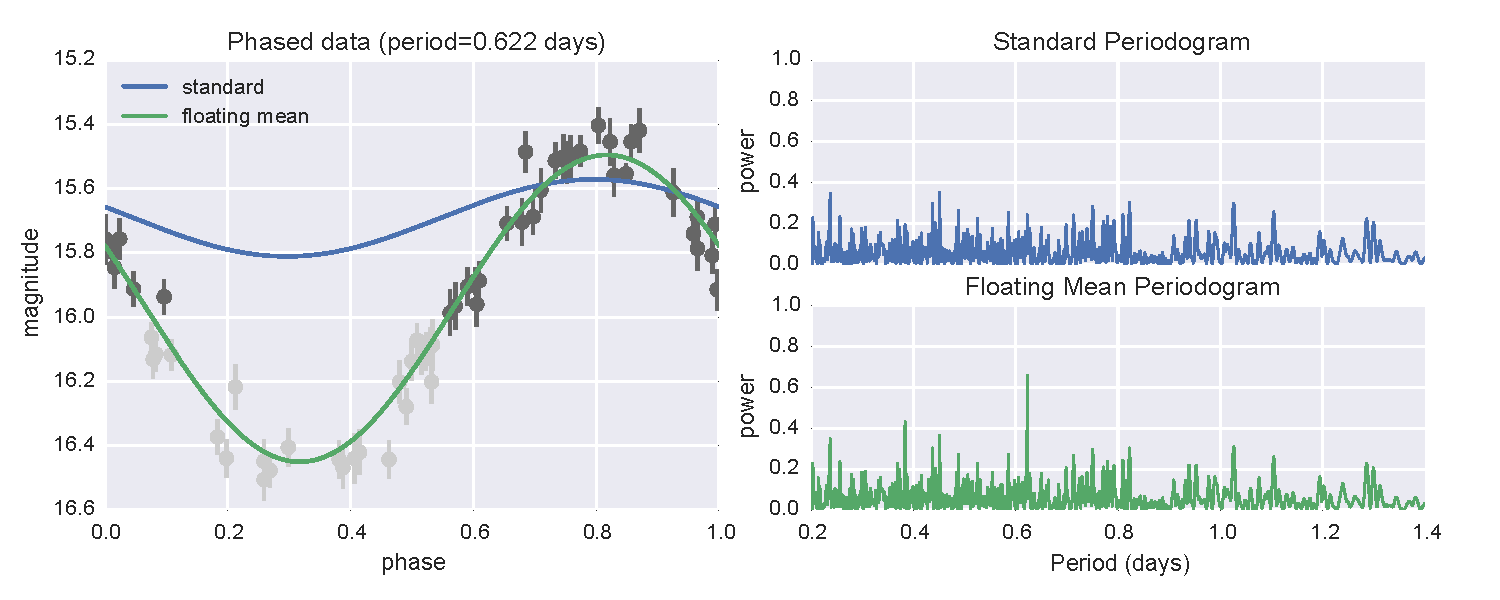
\includegraphics[width=\textwidth]{fig02.pdf}
  \caption{
    Another realization of the data from \fig{01}, with only a single filter
    observed each night (i.e. 12 observations per band, spread over 180
    days). In this case, single-band data is not sufficient to recover the
    Lomb-Scargle peaks, and the classic band-by-band approach fails.
    By utilizing all the data at once with the multiband approach,
    we recover a significant spike of power at the period $P=0.622$ days.    
  } 
  \figlabel{02}
\end{figure}

\begin{itemize}
  \item Show power spectrum for a single-band RR-Lyrae
  \item Reduce observations, show multiple power spectra for multi-band RR-Lyrae
  \item Show single power spectrum for multi-band RR-Lyrae
\end{itemize}

\subsection{Stripe 82}

\begin{itemize}
  \item Compute periods using majority method
  \item Compute periods using unified method
  \item Compare the results
\end{itemize}

\section{Further work}

\begin{itemize}
  \item issues with window function corrections
  \item issues with physicality of model
\end{itemize}


\bibliographystyle{apj}
\bibliography{paper}

%\appendix

\end{document}
